\documentclass[a4paper]{article}
\usepackage[italian]{babel}
\font\TitleFont=cmr12 at 50pt
\font\AuthFont=cmr13 at 20pt
\font\ChapFont=cmr12 at 30 pt
\usepackage{titling}
\usepackage{graphicx}
\usepackage[section]{placeins}
\usepackage{tabularx}

\title {{\TitleFont Esercizio 1}}
\date{3 Luglio 2019}
\author{{\AuthFont Alessandro D'Amico}}


\renewcommand\maketitlehooka{\null\mbox{}\vfill}
\renewcommand\maketitlehookd{\vfill\null}

\begin{document}
\begin{titlingpage}
\maketitle
\end{titlingpage}
\tableofcontents
\newpage
\section{Introduzione al problema}
Nel seguente esperimento viene preso in considerazione il problema dell'ordinamento, per la cui soluzione utilizziamo due differenti algoritmi: Insertion Sort e Merge Sort.
Lo scopo e' ottenere un array (una lista di numeri) i cui elementi che lo compongono (inizialmente disposti in modo casuale) siano disposti in ordine crescente.
\section{Caratteristiche teoriche di algoritmi e e strutture utilizzate}
Insertion
\section{Prestazioni attese}
	\begin{tabularx}{10cm}{|X|X|X|}
	\hline
	Algoritmo & Tempo di esecuzione caso peggiore & Tempo di esecuzione atteso / caso medio \\
	\hline
	\textbf{Insertion Sort} & $\Theta(n^2)$  & $\Theta(n^2)$ \\
	\hline
	\textbf{Merge Sort} &  $\Theta(n\log{}n)$ & $\Theta(n\log{}n)$\\
	\hline
	\end{tabularx}
\section{Esperimenti}
\section{Documentazione del codice}
\newpage
\section{Risultati}
Sono stati effettuati i test con piu set di numeri (set da 10, 100, 1000 valori), tenendo conto del fatto che la dimensione di ogni singolo numero (in termini di cifre) non incide sulla nostra analisi (trattandosi di algoritmi per confronto (non si tiene conto del max o del min). E' dunque necessario distinguere due casi, a seconda che si usi un set ridotto o un set di grandi dimensioni. 
\subsection{Input in ordine crescente}
Dalla Figura \ref{fig:SmallInsMergeCresc} traspare che per ordinare meno di 80 numeri Insertion Sort risulta piu' veloce (cio' e' dovuto principalmente al tempo impiegato al caricamento delle funzioni sulla stack).	

 
		\begin{figure}[!htb]
		\centering
		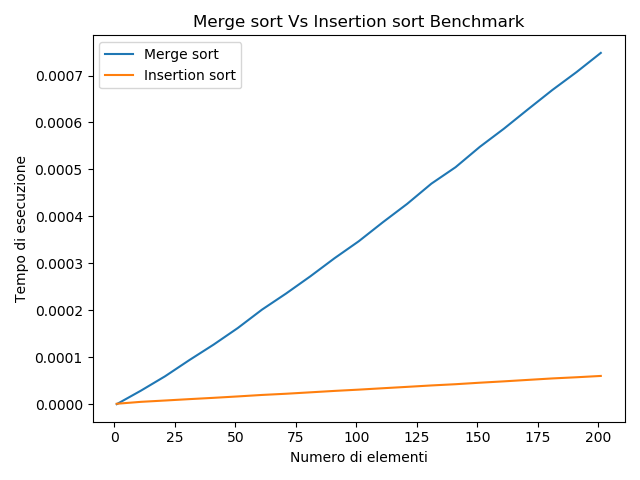
\includegraphics[scale=0.3]{2}
		\caption{Merge Sort vs Insertion Sort per pochi input (ordinati crescentemente)}
		\label{fig:SmallInsMergeCresc}
		\end{figure}
		
		\begin{figure}[!htb]
		\centering
		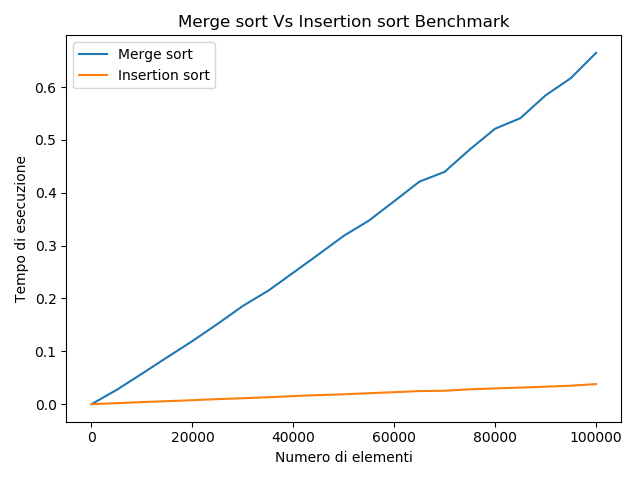
\includegraphics[scale=0.3]{1}
		\caption{Merge Sort vs Insertion Sort per molti input (ordinati crescentemente)}
		\label{fig:BigInsMergeCresc}
		\end{figure}
		

\newpage		
\subsection{Input in ordine decrescente}
Grazie alla figura \ref{fig:BigInsMergeDecr} e' facilmente deducibile che per grandi set di numeri da ordinare Merge Sort  e' sensibilmente piu' rapido rispetto a Insertion Sort 
 
		\begin{figure}[!htb]
		\centering
		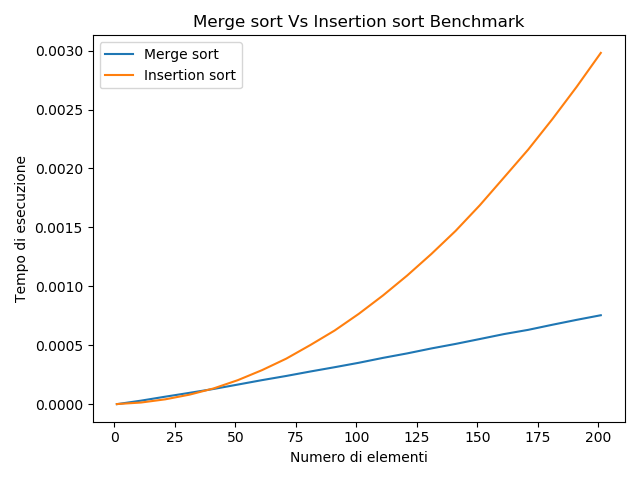
\includegraphics[scale=0.3]{4}
		\caption{Merge Sort vs Insertion Sort per pochi input (ordinati decrescentemente)}
		\label{fig:SmallInsMergeDecr}
		\end{figure}
		
		\begin{figure}[!htb]
		\centering
		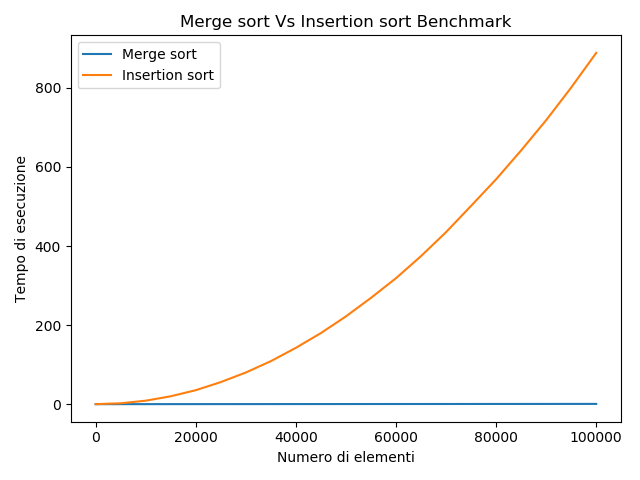
\includegraphics[scale=0.3]{3}
		\caption{Merge Sort vs Insertion Sort per molti input (ordinati decrescentemente)}
		\label{fig:BigInsMergeDecr}
		\end{figure}
\newpage		
\subsection{Input in ordine random}		

		\begin{figure}[!htb]
		\centering
		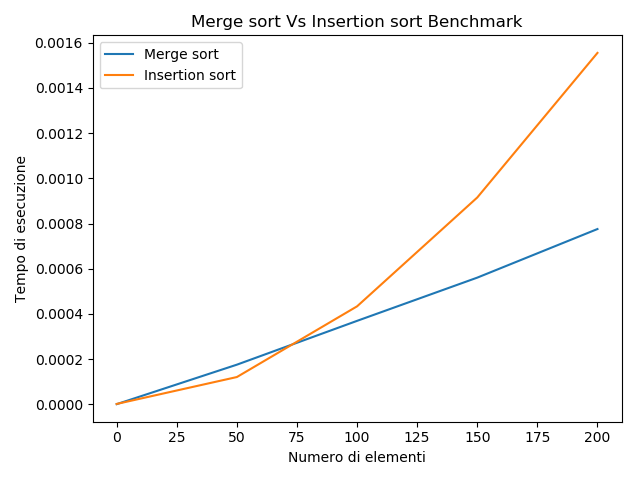
\includegraphics[scale=0.3]{6}
		\caption{Merge Sort vs Insertion Sort per pochi input (random)}
		\label{fig:SmallInsMergeRandom}
		\end{figure}
		
		\begin{figure}[!htb]
		\centering
		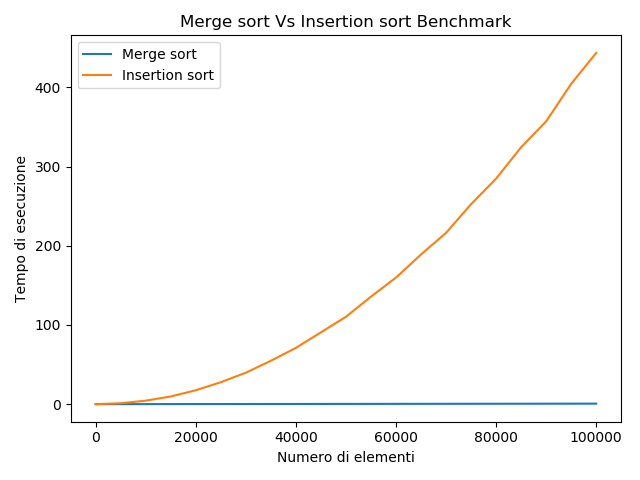
\includegraphics[scale=0.3]{5}
		\caption{Merge Sort vs Insertion Sort per molti input (random)}
		\label{fig:BigInsMergeRandom}
		\end{figure}
		

\section{Conclusioni}
E' stato verificato il comportamento asintotico di Insertion Sort e Merge $\longrightarrow$  \(\infty\)
\end{document}
